\documentclass[
  man,
  floatsintext,
  longtable,
  nolmodern,
  notxfonts,
  notimes,
  colorlinks=true,linkcolor=blue,citecolor=blue,urlcolor=blue]{apa7}

\usepackage{amsmath}
\usepackage{amssymb}




\RequirePackage{longtable}
\RequirePackage{threeparttablex}

\makeatletter
\renewcommand{\paragraph}{\@startsection{paragraph}{4}{\parindent}%
	{0\baselineskip \@plus 0.2ex \@minus 0.2ex}%
	{-.5em}%
	{\normalfont\normalsize\bfseries\typesectitle}}

\renewcommand{\subparagraph}[1]{\@startsection{subparagraph}{5}{0.5em}%
	{0\baselineskip \@plus 0.2ex \@minus 0.2ex}%
	{-\z@\relax}%
	{\normalfont\normalsize\bfseries\itshape\hspace{\parindent}{#1}\textit{\addperi}}{\relax}}
\makeatother




\usepackage{longtable, booktabs, multirow, multicol, colortbl, hhline, caption, array, float, xpatch}
\setcounter{topnumber}{2}
\setcounter{bottomnumber}{2}
\setcounter{totalnumber}{4}
\renewcommand{\topfraction}{0.85}
\renewcommand{\bottomfraction}{0.85}
\renewcommand{\textfraction}{0.15}
\renewcommand{\floatpagefraction}{0.7}

\usepackage{tcolorbox}
\tcbuselibrary{listings,theorems, breakable, skins}
\usepackage{fontawesome5}

\definecolor{quarto-callout-color}{HTML}{909090}
\definecolor{quarto-callout-note-color}{HTML}{0758E5}
\definecolor{quarto-callout-important-color}{HTML}{CC1914}
\definecolor{quarto-callout-warning-color}{HTML}{EB9113}
\definecolor{quarto-callout-tip-color}{HTML}{00A047}
\definecolor{quarto-callout-caution-color}{HTML}{FC5300}
\definecolor{quarto-callout-color-frame}{HTML}{ACACAC}
\definecolor{quarto-callout-note-color-frame}{HTML}{4582EC}
\definecolor{quarto-callout-important-color-frame}{HTML}{D9534F}
\definecolor{quarto-callout-warning-color-frame}{HTML}{F0AD4E}
\definecolor{quarto-callout-tip-color-frame}{HTML}{02B875}
\definecolor{quarto-callout-caution-color-frame}{HTML}{FD7E14}

%\newlength\Oldarrayrulewidth
%\newlength\Oldtabcolsep


\usepackage{hyperref}




\providecommand{\tightlist}{%
  \setlength{\itemsep}{0pt}\setlength{\parskip}{0pt}}
\usepackage{longtable,booktabs,array}
\usepackage{calc} % for calculating minipage widths
% Correct order of tables after \paragraph or \subparagraph
\usepackage{etoolbox}
\makeatletter
\patchcmd\longtable{\par}{\if@noskipsec\mbox{}\fi\par}{}{}
\makeatother
% Allow footnotes in longtable head/foot
\IfFileExists{footnotehyper.sty}{\usepackage{footnotehyper}}{\usepackage{footnote}}
\makesavenoteenv{longtable}

\usepackage{graphicx}
\makeatletter
\newsavebox\pandoc@box
\newcommand*\pandocbounded[1]{% scales image to fit in text height/width
  \sbox\pandoc@box{#1}%
  \Gscale@div\@tempa{\textheight}{\dimexpr\ht\pandoc@box+\dp\pandoc@box\relax}%
  \Gscale@div\@tempb{\linewidth}{\wd\pandoc@box}%
  \ifdim\@tempb\p@<\@tempa\p@\let\@tempa\@tempb\fi% select the smaller of both
  \ifdim\@tempa\p@<\p@\scalebox{\@tempa}{\usebox\pandoc@box}%
  \else\usebox{\pandoc@box}%
  \fi%
}
% Set default figure placement to htbp
\def\fps@figure{htbp}
\makeatother


% definitions for citeproc citations
\NewDocumentCommand\citeproctext{}{}
\NewDocumentCommand\citeproc{mm}{%
  \begingroup\def\citeproctext{#2}\cite{#1}\endgroup}
\makeatletter
 % allow citations to break across lines
 \let\@cite@ofmt\@firstofone
 % avoid brackets around text for \cite:
 \def\@biblabel#1{}
 \def\@cite#1#2{{#1\if@tempswa , #2\fi}}
\makeatother
\newlength{\cslhangindent}
\setlength{\cslhangindent}{1.5em}
\newlength{\csllabelwidth}
\setlength{\csllabelwidth}{3em}
\newenvironment{CSLReferences}[2] % #1 hanging-indent, #2 entry-spacing
 {\begin{list}{}{%
  \setlength{\itemindent}{0pt}
  \setlength{\leftmargin}{0pt}
  \setlength{\parsep}{0pt}
  % turn on hanging indent if param 1 is 1
  \ifodd #1
   \setlength{\leftmargin}{\cslhangindent}
   \setlength{\itemindent}{-1\cslhangindent}
  \fi
  % set entry spacing
  \setlength{\itemsep}{#2\baselineskip}}}
 {\end{list}}
\usepackage{calc}
\newcommand{\CSLBlock}[1]{\hfill\break\parbox[t]{\linewidth}{\strut\ignorespaces#1\strut}}
\newcommand{\CSLLeftMargin}[1]{\parbox[t]{\csllabelwidth}{\strut#1\strut}}
\newcommand{\CSLRightInline}[1]{\parbox[t]{\linewidth - \csllabelwidth}{\strut#1\strut}}
\newcommand{\CSLIndent}[1]{\hspace{\cslhangindent}#1}





\usepackage{newtx}

\defaultfontfeatures{Scale=MatchLowercase}
\defaultfontfeatures[\rmfamily]{Ligatures=TeX,Scale=1}





\title{The Impact of Heat Stress on Reactive Aggression: Exploring the
Roles of Impulsivity and Trait Aggression Moderators}


\shorttitle{Heat Stress and Aggression}


\usepackage{etoolbox}






\author{Chenyi Dai}



\affiliation{
{Department of Psychology, University of Chicago}}




\leftheader{Dai}



\abstract{This study examines the impact of heat stress on reactive
aggression and the moderating roles of impulsivity and trait aggression.
Using a within-subjects, three-session design, participants were exposed
to room temperature (72°F), moderate heat (97°F), and extreme heat
(113°F) while completing the Retaliate or Carry-On: Reactive Aggression
Experiment (RC-RAGE). A significant main effect of temperature was found
for strongly costly retaliation, with participants in the heat condition
exhibiting significantly higher costly retaliation rates than those in
the control and moderate heat conditions. The current data collection is
ongoing; this report mimics the data collection process using simulated
data to establish the planned analytical pipeline and ensure
methodological rigor. }

\keywords{Heat
stress, Aggression, Impulsivity, Retaliation, Mediation, Moderation}

\authornote{ 

\par{       }
\par{Correspondence concerning this article should be addressed
to Chenyi Dai, Email: cydai@uchicago.edu}
}

\makeatletter
\let\endoldlt\endlongtable
\def\endlongtable{
\hline
\endoldlt
}
\makeatother

\urlstyle{same}



\usepackage{booktabs}
\usepackage{longtable}
\usepackage{array}
\usepackage{multirow}
\usepackage{wrapfig}
\usepackage{float}
\usepackage{colortbl}
\usepackage{pdflscape}
\usepackage{tabu}
\usepackage{threeparttable}
\usepackage{threeparttablex}
\usepackage[normalem]{ulem}
\usepackage{makecell}
\usepackage{xcolor}
\makeatletter
\@ifpackageloaded{caption}{}{\usepackage{caption}}
\AtBeginDocument{%
\ifdefined\contentsname
  \renewcommand*\contentsname{Table of contents}
\else
  \newcommand\contentsname{Table of contents}
\fi
\ifdefined\listfigurename
  \renewcommand*\listfigurename{List of Figures}
\else
  \newcommand\listfigurename{List of Figures}
\fi
\ifdefined\listtablename
  \renewcommand*\listtablename{List of Tables}
\else
  \newcommand\listtablename{List of Tables}
\fi
\ifdefined\figurename
  \renewcommand*\figurename{Figure}
\else
  \newcommand\figurename{Figure}
\fi
\ifdefined\tablename
  \renewcommand*\tablename{Table}
\else
  \newcommand\tablename{Table}
\fi
}
\@ifpackageloaded{float}{}{\usepackage{float}}
\floatstyle{ruled}
\@ifundefined{c@chapter}{\newfloat{codelisting}{h}{lop}}{\newfloat{codelisting}{h}{lop}[chapter]}
\floatname{codelisting}{Listing}
\newcommand*\listoflistings{\listof{codelisting}{List of Listings}}
\makeatother
\makeatletter
\makeatother
\makeatletter
\@ifpackageloaded{caption}{}{\usepackage{caption}}
\@ifpackageloaded{subcaption}{}{\usepackage{subcaption}}
\makeatother

% From https://tex.stackexchange.com/a/645996/211326
%%% apa7 doesn't want to add appendix section titles in the toc
%%% let's make it do it
\makeatletter
\xpatchcmd{\appendix}
  {\par}
  {\addcontentsline{toc}{section}{\@currentlabelname}\par}
  {}{}
\makeatother

%% Disable longtable counter
%% https://tex.stackexchange.com/a/248395/211326

\usepackage{etoolbox}

\makeatletter
\patchcmd{\LT@caption}
  {\bgroup}
  {\bgroup\global\LTpatch@captiontrue}
  {}{}
\patchcmd{\longtable}
  {\par}
  {\par\global\LTpatch@captionfalse}
  {}{}
\apptocmd{\endlongtable}
  {\ifLTpatch@caption\else\addtocounter{table}{-1}\fi}
  {}{}
\newif\ifLTpatch@caption
\makeatother

\begin{document}

\maketitle


\setcounter{secnumdepth}{-\maxdimen} % remove section numbering

\setlength\LTleft{0pt}


The physiological mechanisms that discovered the effects of thermal
exposure on human core and skin temperatures were fully explained by
previous literature, with extensive research highlighting how heat
influences psychological and behavioral outcomes. Thermal stress impacts
cognition (\citeproc{ref-hancockEffectsHeatStress2003a}{Hancock \&
Vasmatzidis, 2003}), neurotransmitter activity involving norepinephrine,
dopamine, and serotonin
(\citeproc{ref-lohmusPossibleBiologicalMechanisms2018a}{Lõhmus, 2018}),
stress hormone levels
(\citeproc{ref-brennerStressHormonesImmunological2007a}{Brenner et al.,
2007}), and emotional states
(\citeproc{ref-escobarTemperatureEmotions2021}{Escobar et al., 2021}).
Understanding these effects has taken on heightened importance in the
context of global climate change and rising ambient temperatures.
Elevated temperatures have been associated with increased substance use,
violent crimes such as robbery and homicide
(\citeproc{ref-thomasWeirdWinterWeather2023}{Thomas \& Wolff, 2023};
\citeproc{ref-tomassiniExploringNexusClimate2024}{Tomassini et al.,
2024}), and higher suicide rates: studies suggest that a 1°C rise in air
temperature correlates with an uptick in suicides
(\citeproc{ref-kimAssociationDailyEnvironmental2011}{Y. Kim et al.,
2011}); (\citeproc{ref-burkeHigherTemperaturesIncrease2018}{Burke et
al., 2018}). One established framework is the Heat Hypothesis, proposed
by Anderson (\citeproc{ref-andersonHeatViolence2001a}{2001}), which
posits that high temperatures elevate aggressive motivation and the
likelihood of aggressive behavior. For instance, improved climate
control in institutional settings (e.g., prisons, schools, and the
workplace) has been recommended as a potential strategy to mitigate
aggression (\citeproc{ref-andersonHeatViolence2001a}{Anderson, 2001}).
Additionally, heat stress significantly impacts occupational health and
safety. High temperatures pose physical health risks and impair
cognitive performance, especially in hot work environments
(\citeproc{ref-srinivasanImpactHeatStress2024a}{Srinivasan et al.,
2024}). Workplaces involving complex tasks are particularly vulnerable
to heat-induced declines in productivity and decision-making accuracy
(\citeproc{ref-spectorHeatExposureOccupational2019a}{Spector et al.,
2019}). These findings underscore the importance of investigating the
relationship between heat stress and behavioral and psychological
dysregulation, as this can inform strategies to address mental health
challenges and mitigate aggression-related issues in occupational,
social, and institutional contexts. This study specifically examines the
effects of heat stress on aggression, exploring potential mediating
variables such as cognitive performance, emotional regulation, and
individual differences to better understand the mechanisms driving this
relationship. Investigating these dynamics aims to provide
evidence-based insights that can guide the formulation of policies and
interventions to enhance psychological resilience, reduce aggression,
and improve overall quality of life in the face of challenges posed by
global warming.

Both observational and experimental studies demonstrate a significant
relationship between heat stress and aggression. Observational research,
such as a study examining aggression by assault death data from Seoul,
found that the overall risk of death by assault increased by 1.4\% for
every 1°C rise in ambient temperature
(\citeproc{ref-kimPositiveAssociationAggression2023}{S. E. Kim et al.,
2023}). Experimental findings complement these observations; for
example, Baron and Bell
(\citeproc{ref-baronAggressionHeatInfluence1976}{1976}) found that high
ambient temperatures raised behavioral aggression as participants
delivered stronger electric shocks under heat conditions. Psychological
theories like the Temperature-Aggression Hypothesis
(\citeproc{ref-andersonTemperatureAggression2000}{Anderson et al.,
2000}) support this connection between heat and aggression. This theory
posits that elevated temperatures increase aggressive motivation and,
under conducive circumstances, lead to aggressive behavior. Aggression
can be categorized into two primary types: reactive aggression,
characterized as impulsive and emotionally driven in response to
provocation or frustration, and proactive aggression, which is
calculated, goal-directed, and less tied to emotional states
(\citeproc{ref-poulinReactiveProactiveAggression2000}{Poulin \& Boivin,
2000}). The distinction is critical, as reactive aggression is often
tied to situational factors like environmental stressors, whereas
proactive aggression is primarily influenced by genetic and learned
behaviors. Given its strong ties to emotional and environmental
triggers, this study focuses specifically on reactive aggression taking
heat stress as the input variable, employing the Retaliate or Carry-On:
Reactive Aggression Experiment (RC-RAGE), developed by Meidenbauer et
al.
(\citeproc{ref-meidenbauerCharacterizingRoleImpulsivity2024a}{2024}), to
investigate how rising temperatures influence impulsive,
provocation-driven aggression under controlled experimental conditions.

Meidenbauer et al.
(\citeproc{ref-meidenbauerCharacterizingRoleImpulsivity2024a}{2024})
emphasized the need for tasks that elicit reactive aggression in
experimental settings, especially among socially desirable individuals,
as social desirability skews self-reported and behavioral aggression
measures, a mismatch attributed to test content rather than a common
desirability factor
(\citeproc{ref-vigil-coletImpactSocialDesirability2012}{Vigil-Colet et
al., 2012}). To address this, the RC-RAGE was developed to fill a
methodological gap by offering a reactive aggression metric suitable for
experimental settings, enabling immediate impulsive responses, imposing
a tangible cost to retaliation, and minimizing the influence of social
desirability biases. Findings demonstrated that costly, reactive
aggression is significantly influenced by impulsivity, reflecting a
tendency to act without planning. Building on the Temperature-Aggression
Hypothesis (\citeproc{ref-andersonTemperatureAggression2000}{Anderson et
al., 2000}), which identifies cognitive (e.g., accessibility of
aggressive thoughts), affective (e.g., heightened hostility or anger),
and arousal (e.g., increased heart rate) pathways through which input
variables influence aggression, and the General Aggression Model
(\citeproc{ref-dewallGeneralAggressionModel2011a}{DeWall \& Anderson,
2011}), which highlights the interaction between individual differences
(e.g., impulsivity) and environmental stressors (e.g., heat), this study
incorporates several internal state variables---impulsivity trait,
aggression trait, personality factors, cognitive flexibility, working
memory, emotional clarity and attention, temperature perception, and
substance consumption---as potential mediators to provide a
comprehensive understanding of the heat-aggression process. To better
understand the mechanisms linking heat exposure to aggression, the
current within-subjects, crossover design experiment focuses on
potential mediators such as cognitive flexibility, working memory, and
subjective discomfort because of their established links to aggression
and cognitive performance. For example, neuroticism and extraversion
have direct positive effects on physical aggression
(\citeproc{ref-cavalcantiPersonalityAggressionContribution2016}{Cavalcanti
\& Pimentel, 2016-Jul-Sep}), and neuroticism is associated with greater
discomfort in response to environmental temperature
(\citeproc{ref-kleiderAggressiveShootingBehavior2009}{Kleider \&
Parrott, 2009}; \citeproc{ref-leblancResponseThermalStress2003}{LeBlanc
et al., 2003}). Previous research shows that heat stress impairs working
memory, attention, response speed, and processing speed
(\citeproc{ref-mazloumiEvaluatingEffectsHeat}{Mazloumi et al., n.d.}).
However, cognitive functions largely remain unaffected unless thermal
stress significantly shifts core body temperature away from steady-state
conditions (\citeproc{ref-hancockEffectsHeatStress2003a}{Hancock \&
Vasmatzidis, 2003}). Interestingly, subjective discomfort from heat can
impair cognitive flexibility even when core body temperature and
cortical excitability are unaffected
(\citeproc{ref-gaouaSensoryDispleasureReduces2012a}{Gaoua et al.,
2012}). To isolate the physiological effects of heat stress, this study
will control heat exposure duration to ensure participants maintain
steady-state core temperatures while monitoring subjective discomfort
and skin temperature.

\subsection{Research Question}\label{research-question}

How does heat stress influence reactive aggression, and what role do
moderating variables such as impulsivity and aggression play in this
relationship?

\subsection{Hypothesis}\label{hypothesis}

Heat stress will increase aggression, with the effects being more
pronounced in individuals with high trait impulsivity and high trait
aggression。

\subsection{Methods}\label{sec-methods}

\subsubsection{Experimental Design}\label{experimental-design}

Data will be collected through a three-part, on-site study consisting of
three sessions held at the same time and on the same day of the week,
spaced one week apart. During two sessions, the chamber will be set to
elevated temperatures, while in the other session, it will be set to
room temperature. Participants will sit in a controlled sauna
environment, wearing a bioharness to monitor physiological indicators
such as core body temperature, skin temperature, and heart rate
variability. They will also complete cognitive tasks assessing working
memory (Backward Digit Span task) and cognitive flexibility (Stop Signal
Task), along with a novel task to evaluate reactive aggression (RC-RAGE
task). Prior research has shown that heat stress may impair memory and
cognitive flexibility
(\citeproc{ref-gaouaSensoryDispleasureReduces2012a}{Gaoua et al.,
2012}). This study extends these findings by introducing a novel
paradigm designed to assess provoked aggression in situations where
self-control is required
(\citeproc{ref-meidenbauerCharacterizingRoleImpulsivity2024a}{Meidenbauer
et al., 2024}).

\subsubsection{Participants}\label{participants}

Participant recruitment will occur through the University of Chicago
Research System, Facebook groups, and campus flyers, with eligibility
determined via online pre-screening. Exclusion criteria include chronic
health issues, non-normal vision, non-English speakers, age outside
18-35, and BMI over 35. The pre-screening survey includes the BIS-11
Impulsivity Questionnaire
(\citeproc{ref-pattonFactorStructureBarratt1995a}{Patton et al., 1995}),
BPAQ Aggression Questionnaire
(\citeproc{ref-bussAggressionQuestionnaire1992}{Buss \& Perry, 1992}),
Big Five Inventory--2 Short Form (BFI-2-S)
(\citeproc{ref-sotoShortExtrashortForms2017}{Soto \& John, 2017}),
Clarity and Attention to Emotions Scale
(\citeproc{ref-palmieriMeasuringClarityAttention2009}{Palmieri et al.,
2009}), Temperature Perceptions scale
(\citeproc{ref-wangInterindividualDifferencesMale2020}{Wang et al.,
2020}), and DFAQ-CU Inventory
(\citeproc{ref-cuttlerMeasuringCannabisConsumption2017}{Cuttler \&
Spradlin, 2017}). These questionnaires assess participants' impulsivity,
aggression, facet traits, emotional awareness, thermal comfort, and
cannabis use to provide baseline measures for analyzing how individual
differences in each trait may influence responses under heat stress. The
questionnaire order was randomized through Qualtrics.

\subsubsection{Procedure}\label{procedure}

This study adheres to ethical guidelines approved by the University of
Chicago Institutional Review Board (IRB 19-1977). Before the study,
participants are instructed to refrain from consuming alcohol or using
any drugs for 24 hours. Following the acquisition of informed consent,
participants are instructed to place a bioharness strap with a heart
rate monitor core body temperature sensor under a standardized heat
suit. Participants are seated, and baseline physiological data are
collected for 5 minutes. Participants are then instructed on the tasks
they will complete in the chamber. Participants then enter the heat
chamber where they have been randomly assigned to one of three
temperature conditions: 97°F, 113°F, or room temperature for 50 minutes.
Following a 5-minute heat chamber calibration, participants first
complete the Backward Digit Span task
(\citeproc{ref-wechslerManualWechslerAdult1955}{Wechsler, 1955}), which
assesses working memory by requiring them to recall a series of digits
in reverse order. Participants are presented with a string of numbers,
which they must repeat back in the opposite sequence. Next, participants
complete the Stop Signal Task
(\citeproc{ref-lappinUseDelayedSignal1966}{Lappin \& Eriksen, 1966}),
which evaluates their cognitive flexibility and response inhibition.
They are shown a series of directional arrows and must quickly choose
one of two options based on the arrow's direction. After completing the
cognitive tasks, participants are instructed to take a five-minute
break, during which they are told that a researcher needs to check on
the progress of another participant in a different room. This statement
is intended to lead participants to believe they have been randomly
assigned to the role of the ``gatherer'' in an upcoming game against
another human player assigned to the role of the ``robber''. The
deception is crucial for maintaining the integrity of the measurement of
reactive aggression. In the RC-RAGE task, participants spend 12 minutes
maximizing their earnings by collecting ``apples'' toward a ``harvest''
of 10 apples (10 apples = 10 cents), while dealing with a ``robber'' who
occasionally steals 5 cents. Participants can either retaliate by
shooting (regaining 3 cents but resetting progress) or continue
collecting while ignoring the robber. Retaliation costs vary based on
progress: advantageous (retaliation at 1-2 clicks), modestly costly
(retaliation at 3-4 clicks), or strongly costly (retaliation at 6-7
clicks). Participants are informed on the best strategy of retaliation
to maximize gains.

\subsubsection{Statistical analysis}\label{statistical-analysis}

The analysis plan followed a multi-step approach. Initially, descriptive
statistics were computed to summarize key variables, including
retaliation rates across temperature conditions and individual
difference measures (impulsivity, aggression, and affect). This provided
an overview of the dataset and informed subsequent analyses (See
Table~\ref{tbl-descriptive-stats}). Additionally, a gender distribution
analysis was conducted to determine whether the dataset allows for
meaningful sex-based comparisons (See
Table~\ref{tbl-gender-distribution}). Visualization techniques were
applied to explore the distribution of retaliation types under different
conditions (See Figure~\ref{fig-costly-retaliation-facet}).

To test whether heat stress increases costly retaliation, a series of
one-way ANOVAs were conducted separately for modestly costly and
strongly costly retaliation rates. These models assessed whether
retaliation rates significantly differed between control, moderate, and
high-temperature conditions (See Table~\ref{tbl-anova-modestly-table};
See Table~\ref{tbl-anova-strongly-table}). Significant findings would
suggest that temperature exposure influences aggressive responses.

To investigate the role of individual differences, a logistic
mixed-effects regression model was estimated to predict strongly costly
retaliation. The predictors included temperature condition, trait
impulsivity (BISTotal), and trait aggression (BPAQTotal), while
controlling for repeated measures within participants (random intercept:
ID). This model addressed the question: Do personality traits influence
retaliation tendencies under different temperature conditions? (See
Table~\ref{tbl-logit-table}).

Given previous research suggesting that impulsivity and aggression may
moderate the effects of heat stress on aggression, a series of
moderation models were then tested:

\begin{enumerate}
\def\labelenumi{\arabic{enumi}.}
\tightlist
\item
  \emph{Overall Moderation Model:} Examined whether overall impulsivity
  (BISTotal) and aggression (BPAQTotal) moderated the effect of
  temperature on strongly costly retaliation.
\item
  \emph{BIS Subscale Moderation:} Tested whether specific facets of
  impulsivity (BIS Attentional, BIS Motor, BIS Nonplanning) interacted
  with temperature condition to influence retaliation.
\item
  \emph{BPAQ Subscale Moderation:} Investigated whether different
  aspects of aggression (BPAQ Physical, BPAQ Verbal, BPAQ Anger, BPAQ
  Hostility) modified the temperature-aggression relationship.
\item
  \emph{Combined Moderation Model:} Simultaneously tested all
  impulsivity and aggression subscales to determine their collective
  moderating effect.
\end{enumerate}

These models assessed whether certain personality traits increase
susceptibility to aggression under heat stress.

Finally, a correlational analysis was conducted to examine the
relationship between negative affect (PANASNA scores) and strongly
costly retaliation rates within each temperature condition. A
significant correlation would suggest that heightened negative affect
might mediate the relationship between heat stress and aggression (See
Figure~\ref{fig-scatter-panasna}).

\subsection{Results}\label{results}

\subsubsection{Descriptive Statistics and Preliminary
Analyses}\label{descriptive-statistics-and-preliminary-analyses}

Descriptive statistics for key variables are presented in
Table~\ref{tbl-descriptive-stats}. The mean level of two types of costly
retaliation across all conditions was 0.99, with a standard deviation of
0.64. Negative affect scores (PANASNA) had a mean of 20.75 (SD = 2.06).

The sample was highly skewed towards female participants, with 108
females (representing 72\%) and 42 males (28\%). Given the imbalance,
gender effects should be interpreted cautiously.

\begin{figure}

\caption{\label{fig-costly-retaliation-facet}Retaliation Rates Across
Temperature Conditions}

\centering{

\pandocbounded{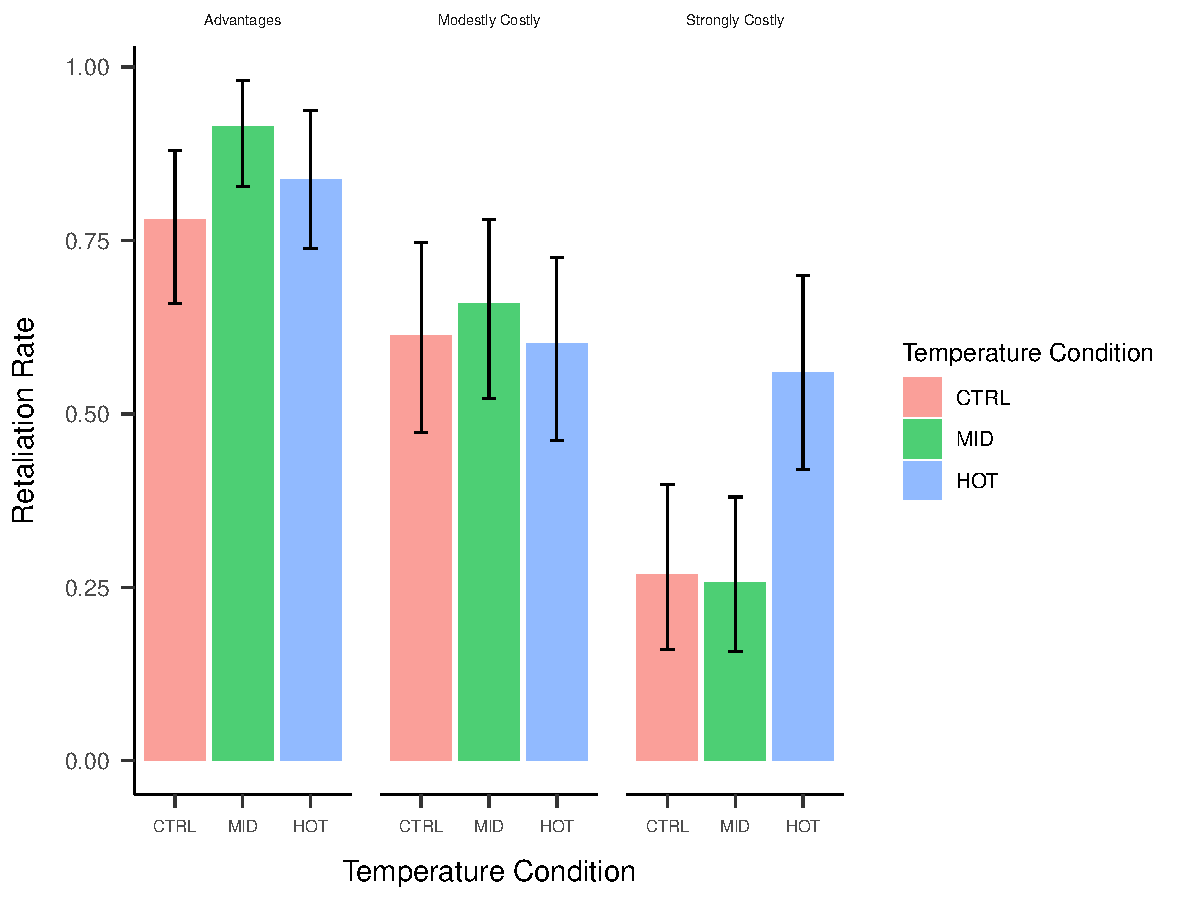
\includegraphics[keepaspectratio]{manuscript_files/figure-pdf/fig-costly-retaliation-facet-1.pdf}}

}

\end{figure}%

\begin{table}

{\caption{{Descriptive Statistics for Key
Variables}{\label{tbl-descriptive-stats}}}
\vspace{-20pt}}

\centering
\begin{tabular}[t]{l|r|r}
\hline
Variable & Mean & SD\\
\hline
Costly Retaliation & 0.99 & 0.64\\
\hline
Negative Affect (PANASNA) & 20.75 & 2.06\\
\hline
Novaco Anger & 18.10 & 3.43\\
\hline
Trait Aggression (BPAQ) & 175.72 & 16.02\\
\hline
Trait Impulsivity (BIS) & 151.36 & 10.42\\
\hline
\end{tabular}

\end{table}

\begin{table}

{\caption{{Descriptive Statistics for Gender
Distrivution}{\label{tbl-gender-distribution}}}
\vspace{-20pt}}

\centering
\begin{tabular}[t]{l|r|r}
\hline
gender & Count & Proportion\\
\hline
Female & 36 & 0.72\\
\hline
Male & 14 & 0.28\\
\hline
\end{tabular}

\end{table}

\begin{table}

{\caption{{One-Way ANOVA for Modestly Costly
Retaliation}{\label{tbl-anova-modestly-table}}}
\vspace{-20pt}}

\centering
\begin{tabular}[t]{lrrrll}
\toprule
Source & df & Sum of Squares & Mean Square & F & p\\
\midrule
Temperature Condition & 2 & 0.092 & 0.046 & 0.196 & 0.823\\
Error & 147 & 34.398 & 0.234 & -- & --\\
\bottomrule
\end{tabular}

\end{table}

\begin{table}

{\caption{{One-Way ANOVA for Stongly Costly
Retaliation}{\label{tbl-anova-strongly-table}}}
\vspace{-20pt}}

\centering\centering
\resizebox{\ifdim\width>\linewidth\linewidth\else\width\fi}{!}{
\begin{tabular}[t]{lrrrll}
\toprule
Source & df & Sum of Squares & Mean Square & F & p\\
\midrule
Temperature Condition & 2 & 2.941 & 1.470 & 6.905 & 0.001\\
Error & 147 & 31.300 & 0.213 & -- & --\\
\bottomrule
\multicolumn{6}{l}{\rule{0pt}{1em}Note. df = degrees of freedom. F and p are not computed for the Error row.}\\
\end{tabular}}

\end{table}

\subsubsection{ANOVA Results}\label{anova-results}

Figure~\ref{fig-costly-retaliation-facet} presents the retaliation rates
across temperature conditions, separated by retaliation type
(Advantageous, Modestly Costly, and Strongly Costly). The visualization
suggests that participants in the HOT condition exhibit a higher
proportion of strongly costly retaliation compared to those in the CTRL
and MID conditions. In contrast, retaliation classified as modestly
costly appeared to be more evenly distributed across temperature
conditions, suggesting a less pronounced effect of heat stress in this
category. The error bars, reflecting 95\% confidence intervals, indicate
greater variability in strongly costly retaliation under
high-temperature exposure.

Separate one-way ANOVAs were conducted to examine the effects of
temperature condition on costly retaliation measures and to
statistically evaluate these observations. The analysis for modestly
costly retaliation (See Table~\ref{tbl-anova-modestly-table}) did not
reveal a significant main effect of temperature condition, F = 0.196,
\emph{p} = 0.823, suggesting that exposure to elevated temperatures did
not significantly influence engagement in modestly costly retaliation.
In contrast, the ANOVA for strongly costly retaliation (See
Table~\ref{tbl-anova-strongly-table}) yielded a statistically
significant effect of temperature condition, F = 6.905, \emph{p} =
0.001, indicating that higher temperatures significantly increased the
likelihood of engaging in strongly costly retaliation. Overall, the
results indicate that exposure to extreme heat significantly increases
engagement in strongly costly retaliation, whereas modestly costly
retaliation remains unaffected by temperature variations. The lack of
significant differences between the MID and CTRL conditions suggests
that moderate increases in temperature do not elicit the same elevation
in aggression as higher heat exposure. Future research should explore
potential mediating mechanisms, such as body temperature, heart rate
variability, or cognitive control, to further explore the relationship
between thermal stress and aggressive decision-making.

\begin{table}

{\caption{{Logistic Mixed Model Fixed Effects
Estimates}{\label{tbl-logit-table}}}
\vspace{-20pt}}

\centering
\begin{tabular}[t]{>{}lrrlrl}
\toprule
Predictor & B & SE & CI & z-value & p-value\\
\midrule
\textbf{Intercept} & 0.484 & 3.432 & {}[-6.243, 7.21] & 0.141 & 0.888\\
\textbf{Temperature (MID vs. CTRL)} & -0.064 & 0.463 & {}[-0.973, 0.844] & -0.139 & 0.889\\
\textbf{Temperature (HOT vs. CTRL)} & 1.297 & 0.439 & {}[0.437, 2.158] & 2.954 & 0.003\\
\textbf{Trait Impulsivity (BIS)} & 0.019 & 0.018 & {}[-0.016, 0.054] & 1.042 & 0.297\\
\textbf{Trait Aggression (BPAQ)} & -0.025 & 0.012 & {}[-0.047, -0.002] & -2.146 & 0.032\\
\bottomrule
\multicolumn{6}{l}{\rule{0pt}{1em}\textit{Model 1: Temperature, Impulsivity, and Aggression as Predictors of Strongly Costly Retaliation}}\\
\multicolumn{6}{l}{\rule{0pt}{1em}Note. B = logit coefficient, SE = standard error, z = test statistic, p = p-value, 95\% CI in brackets.}\\
\end{tabular}

\end{table}

\subsubsection{Logistic Mixed-Effects
Modeling}\label{logistic-mixed-effects-modeling}

A logistic mixed-effects model was conducted to examine the effects of
temperature condition, trait impulsivity (BIS), and trait aggression
(BPAQ) on the likelihood of engaging in strongly costly retaliation. The
model included temperature condition, BIS, and BPAQ as fixed effects,
with a random intercept for participant ID to account for repeated
measures. The results are presented in Table~\ref{tbl-logit-table}. The
analysis revealed that participants in the HOT condition exhibited a
significantly higher likelihood of engaging in strongly costly
retaliation compared to those in the CTRL condition, B = 1.297, SE =
0.439, z = 2.954, \emph{p} = 0.00314. The 95\% confidence interval (CI)
for this effect ranged from 0.437 to 2.158, suggesting a robust effect
of high-temperature exposure on retaliatory aggression. This finding is
consistent with the previous results from one-way ANOVA. In contrast, no
significant difference was observed between the MID and CTRL conditions,
\emph{p} = 0.889, indicating that moderate heat stress did not
significantly alter retaliatory behavior. This suggests a threshold
effect, where only extreme heat exposure substantially increases
aggressive responses.

Trait aggression (BPAQ) was also a significant predictor of strongly
costly retaliation, B = -0.025, \emph{p} = 0.0319, indicating that
individuals higher in trait aggression were more likely to retaliate
under costly conditions. The 95\% CI for this effect ranged from -0.047
to -0.002, suggesting that aggression-related personality traits play a
meaningful role in shaping retaliatory decisions. However, trait
impulsivity (BIS) did not exhibit a significant main effect, \emph{p} =
0.297, suggesting that impulsivity alone was not a strong predictor of
costly retaliation in the current model. This finding contrasts with
previous literature linking impulsivity to heightened aggression,
raising the possibility that impulsivity's influence on retaliation may
depend on specific contextual or interactive factors, such as emotional
state or provocation intensity.

These findings highlight the complex interplay between environmental
stressors and individual traits in predicting retaliatory aggression.
While extreme heat exposure independently heightened aggression, its
effects were amplified among individuals high in trait aggression.
Future research should explore potential underlying mechanisms, such as
physiological arousal, self-regulation deficits, or emotional
dysregulation, to further elucidate the pathways linking heat exposure
to aggressive decision-making.

\paragraph{Moderation Analyses.}\label{moderation-analyses}

The moderation analysis tested whether trait impulsivity (BIS) and trait
aggression (BPAQ) moderated the relationship between temperature
condition and strongly costly retaliation. However, as this analysis was
conducted on simulated data, the model fit was relatively low (AIC =
189.3, BIC = 219.4), limiting the reliability of these results. The
model estimates suggest that trait aggression (BPAQ) approached
significance (B = -0.025, p = 0.0319), suggesting a potential negative
relationship. However, the confidence interval () likely includes zero,
which is opposite to theoretical expectations, making it difficult to
draw meaningful conclusions.

Given these limitations, no additional visualizations or in-depth
interpretations were included for this model. Instead, subsequent
analyses focus on breaking down impulsivity and aggression into
subcomponents to better understand potential nuanced interactions, as
well as investigating negative affect (PANASNA) as a possible mediating
variable in the heat-aggression relationship.

\begin{figure}

\caption{\label{fig-scatter-panasna}Relationship Between Negative Affect
and Temperatur}

\centering{

\pandocbounded{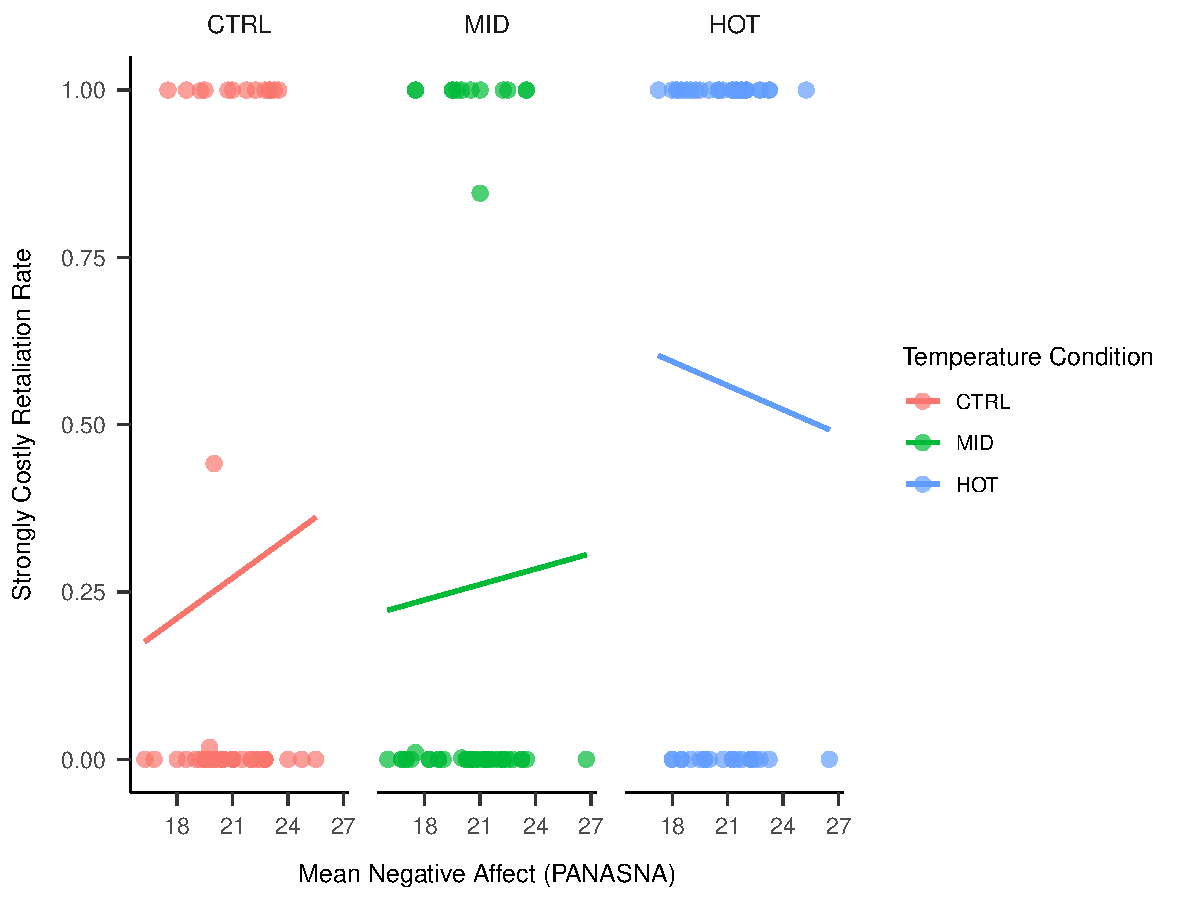
\includegraphics[keepaspectratio]{manuscript_files/figure-pdf/fig-scatter-panasna-1.pdf}}

}

\end{figure}%

\subsubsection{Relationship Between Negative Affect and
Aggression}\label{relationship-between-negative-affect-and-aggression}

A further exploratory visualization serves as a preliminary step for a
mediation analysis investigating whether heat stress increases negative
affect and whether negative affect mediates the relationship between
temperature and aggression. Understanding this relationship is crucial
in determining whether heightened emotional distress is a key driver of
heat-induced aggression rather than direct physiological or cognitive
changes.

Figure~\ref{fig-scatter-panasna} presents a scatterplot depicting the
relationship between mean negative affect (PANASNA) and strongly costly
retaliation, stratified by temperature condition. The observed patterns
indicate potential temperature-dependent associations between negative
affect and aggression.

In the HOT condition, a negative association is observed, suggesting
that participants with higher negative affect exhibited reduced strongly
costly retaliation. This unexpected trend challenges the assumption that
heightened negative emotions under heat stress universally lead to more
aggression, possibly indicating emotion regulation mechanisms or
individual variability in coping strategies under extreme stress.
However, it is important to note that in the current simulated dataset,
PANAS negative affect scores were randomly generated, meaning the
observed pattern may not reflect a true psychological effect. Future
analyses using real datasets will follow this same data analysis
pipeline to assess the actual impact of heat exposure on affective
states and aggression. In contrast, the MID and CTRL conditions show a
positive association between negative affect and aggression.

These preliminary findings imply the complex interplay between affective
states and aggressive behavior under varying temperature conditions.
Given the mixed directional effects, further investigation is warranted
to determine whether negative affect mediates the relationship between
heat stress and aggression.

\subsection{Discussion}\label{discussion}

The present study examined the relationship between heat stress and
reactive aggression, with a particular focus on the moderating role of
individual differences in impulsivity and aggression and the potential
mediating role of negative affect. Using a simulated dataset, the
analyses followed a systematic approach to assess the effects of
temperature on costly retaliation, the interaction between personality
traits and heat exposure, and the role of negative affect in shaping
aggressive responses. In line with the Temperature-Aggression Hypothesis
(\citeproc{ref-andersonTemperatureAggression2000}{Anderson et al.,
2000}), current findings indicate that exposure to high temperatures
significantly increases the likelihood of engaging in aggressive
behavior. Specifically, participants in the HOT condition retaliated
more vigorously compared to their counterparts in the room temperature
and moderately heated (MID) conditions.

While the current study provides a systematic framework for analyzing
heat stress and aggression, several limitations must be acknowledged.
First, the use of a simulated dataset prevents any definitive
conclusions regarding the real-world psychological effects of
temperature on aggression. The results, particularly those related to
negative affect and trait moderation effects, are likely artifacts of
the simulated data structure rather than reflections of true
psychological processes. Additionally, the low model fit and singular
variance estimates in the mixed-effects models indicate that future
studies should incorporate larger sample sizes and more diverse trait
distributions to enhance the robustness of statistical conclusions.

This study established a data analysis pipeline for investigating the
effects of heat stress on aggression, integrating moderation and
mediation analyses to examine the role of personality traits and
negative affect. Although the current findings are constrained by the
limitations of simulated data, the framework provides a strong
foundation for future empirical investigations. The results underscore
the importance of considering both situational and dispositional factors
in understanding aggression under heat stress and highlight the need for
further research using real-world data to clarify these complex
interactions

\clearpage

\subsection{References}\label{references}

\phantomsection\label{refs}
\begin{CSLReferences}{1}{0}
\bibitem[\citeproctext]{ref-andersonHeatViolence2001a}
Anderson, C. A. (2001). Heat and {Violence}. \emph{Current Directions in
Psychological Science}, \emph{10}(1), 33--38.
\url{https://doi.org/10.1111/1467-8721.00109}

\bibitem[\citeproctext]{ref-andersonTemperatureAggression2000}
Anderson, C. A., Anderson, K. B., Dorr, N., DeNeve, K. M., \& Flanagan,
M. (2000). Temperature and aggression. In \emph{Advances in
{Experimental Social Psychology}} (Vol. 32, pp. 63--133). Academic
Press. \url{https://doi.org/10.1016/S0065-2601(00)80004-0}

\bibitem[\citeproctext]{ref-baronAggressionHeatInfluence1976}
Baron, R. A., \& Bell, P. A. (1976). Aggression and heat: {The}
influence of ambient temperature, negative affect, and a cooling drink
on physical aggression. \emph{Journal of Personality and Social
Psychology}, \emph{33}(3), 245--255.
\url{https://doi.org/10.1037/0022-3514.33.3.245}

\bibitem[\citeproctext]{ref-brennerStressHormonesImmunological2007a}
Brenner, I., Shek, P. N., Zamecnik, J., \& Shephard, R. J. (2007).
Stress {Hormones} and the {Immunological Responses} to {Heat} and
{Exercise}. \emph{International Journal of Sports Medicine}, \emph{19},
130--143. \url{https://doi.org/10.1055/s-2007-971895}

\bibitem[\citeproctext]{ref-burkeHigherTemperaturesIncrease2018}
Burke, M., González, F., Baylis, P., Heft-Neal, S., Baysan, C., Basu,
S., \& Hsiang, S. (2018). Higher temperatures increase suicide rates in
the {United States} and {Mexico}. \emph{Nature Climate Change},
\emph{8}(8), 723--729. \url{https://doi.org/10.1038/s41558-018-0222-x}

\bibitem[\citeproctext]{ref-bussAggressionQuestionnaire1992}
Buss, A. H., \& Perry, M. (1992). The {Aggression Questionnaire}.
\emph{Journal of Personality and Social Psychology}, \emph{63}(3),
452--459. \url{https://doi.org/10.1037/0022-3514.63.3.452}

\bibitem[\citeproctext]{ref-cavalcantiPersonalityAggressionContribution2016}
Cavalcanti, J. G., \& Pimentel, C. E. (2016-Jul-Sep). Personality and
aggression: {A} contribution of the {General Aggression Model}.
\emph{Estudos de Psicologia (Campinas)}, \emph{33}, 443--451.
\url{https://doi.org/10.1590/1982-02752016000300008}

\bibitem[\citeproctext]{ref-cuttlerMeasuringCannabisConsumption2017}
Cuttler, C., \& Spradlin, A. (2017). Measuring cannabis consumption:
{Psychometric} properties of the {Daily Sessions}, {Frequency}, {Age} of
{Onset}, and {Quantity} of {Cannabis Use Inventory} ({DFAQ-CU}).
\emph{PLOS ONE}, \emph{12}(5), e0178194.
\url{https://doi.org/10.1371/journal.pone.0178194}

\bibitem[\citeproctext]{ref-dewallGeneralAggressionModel2011a}
DeWall, C. N., \& Anderson, C. A. (2011). The general aggression model.
In \emph{Human aggression and violence: {Causes}, manifestations, and
consequences} (pp. 15--33). American Psychological Association.
\url{https://doi.org/10.1037/12346-001}

\bibitem[\citeproctext]{ref-escobarTemperatureEmotions2021}
Escobar, F. B., Velasco, C., Motoki, K., Byrne, D. V., \& Wang, Q. J.
(2021). The temperature of emotions. \emph{PLOS ONE}, \emph{16}(6),
e0252408. \url{https://doi.org/10.1371/journal.pone.0252408}

\bibitem[\citeproctext]{ref-gaouaSensoryDispleasureReduces2012a}
Gaoua, N., Grantham, J., Racinais, S., \& El Massioui, F. (2012).
Sensory displeasure reduces complex cognitive performance in the heat.
\emph{Journal of Environmental Psychology}, \emph{32}(2), 158--163.
\url{https://doi.org/10.1016/j.jenvp.2012.01.002}

\bibitem[\citeproctext]{ref-hancockEffectsHeatStress2003a}
Hancock, P. A., \& Vasmatzidis, I. (2003). Effects of heat stress on
cognitive performance: The current state of knowledge.
\emph{International Journal of Hyperthermia}, \emph{19}(3), 355--372.
\url{https://doi.org/10.1080/0265673021000054630}

\bibitem[\citeproctext]{ref-kimPositiveAssociationAggression2023}
Kim, S. E., Kim, Y., Hashizume, M., Honda, Y., Kazutaka, O., Hijioka,
Y., \& Kim, H. (2023). Positive {Association} of {Aggression} with
{Ambient Temperature}. \emph{The Yale Journal of Biology and Medicine},
\emph{96}(2), 189--196. \url{https://doi.org/10.59249/RXZX5728}

\bibitem[\citeproctext]{ref-kimAssociationDailyEnvironmental2011}
Kim, Y., Kim, H., \& Kim, D.-S. (2011). Association between daily
environmental temperature and suicide mortality in {Korea} (2001--2005).
\emph{Psychiatry Research}, \emph{186}(2), 390--396.
\url{https://doi.org/10.1016/j.psychres.2010.08.006}

\bibitem[\citeproctext]{ref-kleiderAggressiveShootingBehavior2009}
Kleider, H. M., \& Parrott, D. J. (2009). Aggressive shooting behavior:
{How} working memory and threat influence shoot decisions. \emph{Journal
of Research in Personality}, \emph{43}(3), 494--497.
\url{https://doi.org/10.1016/j.jrp.2008.12.007}

\bibitem[\citeproctext]{ref-lappinUseDelayedSignal1966}
Lappin, J. S., \& Eriksen, C. W. (1966). Use of a delayed signal to stop
a visual reaction-time response. \emph{Journal of Experimental
Psychology}, \emph{72}(6), 805--811.
\url{https://doi.org/10.1037/h0021266}

\bibitem[\citeproctext]{ref-leblancResponseThermalStress2003}
LeBlanc, J., Ducharme, M. B., Pasto, L., \& Thompson, M. (2003).
Response to thermal stress and personality. \emph{Physiology \&
Behavior}, \emph{80}(1), 69--74.
\url{https://doi.org/10.1016/S0031-9384(03)00225-7}

\bibitem[\citeproctext]{ref-lohmusPossibleBiologicalMechanisms2018a}
Lõhmus, M. (2018). Possible {Biological Mechanisms Linking Mental
Health} and {Heat}---{A Contemplative Review}. \emph{International
Journal of Environmental Research and Public Health}, \emph{15}(7),
1515. \url{https://doi.org/10.3390/ijerph15071515}

\bibitem[\citeproctext]{ref-mazloumiEvaluatingEffectsHeat}
Mazloumi, A., Golbabaei, F., Khani, S. M., Kazemi, Z., Hosseini, M.,
Abbasinia, M., \& Dehghan, S. F. (n.d.). Evaluating {Effects} of {Heat
Stress} on {Cognitive Function} among {Workers} in a {Hot Industry}.
\emph{Health Promotion Perspectives}, \emph{4}(2), 240--246.
\url{https://doi.org/10.5681/hpp.2014.031}

\bibitem[\citeproctext]{ref-meidenbauerCharacterizingRoleImpulsivity2024a}
Meidenbauer, K. L., Choe, K. W., Bakkour, A., Inzlicht, M., Meidenbauer,
M. L., \& Berman, M. G. (2024). Characterizing the role of impulsivity
in costly, reactive aggression using a novel paradigm. \emph{Behavior
Research Methods}, \emph{56}(2), 690--708.
\url{https://doi.org/10.3758/s13428-023-02066-9}

\bibitem[\citeproctext]{ref-palmieriMeasuringClarityAttention2009}
Palmieri, P. A., Boden, M. T., \& Berenbaum, H. (2009). Measuring
{Clarity} of and {Attention} to {Emotions}. \emph{Journal of Personality
Assessment}, \emph{91}(6), 560--567.
\url{https://doi.org/10.1080/00223890903228539}

\bibitem[\citeproctext]{ref-pattonFactorStructureBarratt1995a}
Patton, J. H., Stanford, M. S., \& Barratt, E. S. (1995). Factor
structure of the barratt impulsiveness scale. \emph{Journal of Clinical
Psychology}, \emph{51}(6), 768--774.
\url{https://doi.org/10.1002/1097-4679(199511)51:6\%3C768::AID-JCLP2270510607\%3E3.0.CO;2-1}

\bibitem[\citeproctext]{ref-poulinReactiveProactiveAggression2000}
Poulin, F., \& Boivin, M. (2000). Reactive and proactive aggression:
{Evidence} of a two-factor model. \emph{Psychological Assessment},
\emph{12}(2), 115--122. \url{https://doi.org/10.1037/1040-3590.12.2.115}

\bibitem[\citeproctext]{ref-sotoShortExtrashortForms2017}
Soto, C. J., \& John, O. P. (2017). Short and extra-short forms of the
{Big Five Inventory}--2: {The BFI-2-S} and {BFI-2-XS}. \emph{Journal of
Research in Personality}, \emph{68}, 69--81.
\url{https://doi.org/10.1016/j.jrp.2017.02.004}

\bibitem[\citeproctext]{ref-spectorHeatExposureOccupational2019a}
Spector, J. T., Masuda, Y. J., Wolff, N. H., Calkins, M., \& Seixas, N.
(2019). Heat {Exposure} and {Occupational Injuries}: {Review} of the
{Literature} and {Implications}. \emph{Current Environmental Health
Reports}, \emph{6}(4), 286--296.
\url{https://doi.org/10.1007/s40572-019-00250-8}

\bibitem[\citeproctext]{ref-srinivasanImpactHeatStress2024a}
Srinivasan, K., Boulton, C. G., Bhattacharjee, M., Sinha, A.,
Loganathan, S., Seethy, A., Alam, S. M., \& Hanse, B. (2024). Impact of
heat stress on thermal balance, hydration and cortical response among
outdoor workers in hot environment -- an exploratory report from {North
East India}. \emph{Journal of Basic and Clinical Physiology and
Pharmacology}, \emph{35}(1-2), 79--84.
\url{https://doi.org/10.1515/jbcpp-2024-0003}

\bibitem[\citeproctext]{ref-thomasWeirdWinterWeather2023}
Thomas, C., \& Wolff, K. T. (2023). Weird winter weather in the
{Anthropocene}: {How} volatile temperatures shape violent crime.
\emph{Journal of Criminal Justice}, \emph{87}, 102090.
\url{https://doi.org/10.1016/j.jcrimjus.2023.102090}

\bibitem[\citeproctext]{ref-tomassiniExploringNexusClimate2024}
Tomassini, L., Lancia, M., Gambelunghe, A., Zahar, A., Pini, N., \&
Gambelunghe, C. (2024). Exploring the {Nexus} of {Climate Change} and
{Substance Abuse}: {A Scoping Review}. \emph{International Journal of
Environmental Research and Public Health}, \emph{21}(7).
\url{https://doi.org/10.3390/ijerph21070896}

\bibitem[\citeproctext]{ref-vigil-coletImpactSocialDesirability2012}
Vigil-Colet, A., Ruiz-Pamies, M., Anguiano-Carrasco, C., \&
Lorenzo-Seva, U. (2012).
\href{https://www.ncbi.nlm.nih.gov/pubmed/22420362}{The impact of social
desirability on psychometric measures of aggression}. \emph{Psicothema},
\emph{24}(2), 310--315.

\bibitem[\citeproctext]{ref-wangInterindividualDifferencesMale2020}
Wang, L., Chen, M., \& Yang, J. (2020). Interindividual differences of
male college students in thermal preference in winter. \emph{Building
and Environment}, \emph{173}, 106744.
\url{https://doi.org/10.1016/j.buildenv.2020.106744}

\bibitem[\citeproctext]{ref-wechslerManualWechslerAdult1955}
Wechsler, D. (1955). \emph{Manual for the {Wechsler Adult Intelligence
Scale}} (pp. vi, 110). Psychological Corp.

\end{CSLReferences}






\end{document}
